\chapter{MC-SBD-STM Performance}

\section{Synthetic Data Generation Process}
\subsection{Shortcomings of existing algorithm}
\begin{itemize}
	\item 1. Their simulation data used truncated QPI pattern, not true to the real STM case. 
	\item 2. Too ideal to be useful in most cases,
\end{itemize}

Shortcoming in generating the observations. The purpose here is to simulate as close to experiment as possible to test and benchmark this method. 

I would like to elaborate on the truncation they made, they are given a simulation result, say a $256\times256\times41$ of $\delta\rho$ covering say 50 by 50 lattice from single defect at the center, without considering the noise level, the authors truncate the initial 50 by 50 lattice down to 19 by 19. In the generation of the observation, a parameter is set to be the ratio between the kernel size versus the window size, by setting this, they determined target size of the kernel in pixel, and then they can reshape the 19 by 19 lattice simulation into the target size. While one can argue that this process of truncating and reshape did not hinder the purpose of testing the SBD algorithm. It fails to simulate what happened in the experiment. Note that with this method, the boundary of the real-space QPI pattern is artificially set by the truncation.

Physically, the boundary of real-space QPI pattern is resulted from the interplay between the quasiparticle lifetime and the noise level, as kind of illustrated in Fig. \ref{fig:ch5_cutoff}; Thus, the kernel-window size ratio can be calculated after setting up the designed noise level at an energy slice, and due to this direct correlation, we argue that this is not a well-defined free parameter to be considered in the simulation. 

The way they simulate the observation is through the 2D convolution between a reshaped kernel with QPI pattern and an ideally binary activation; The convolution thus enforced defects sitting at activation pixels with entry equal to one. As defects can only site on the lattice sites, this only make sense when we define the activation map as the lattice site, which is not how it is defined in this work. 

The conflict here is that we need 2 uncorrelated free parameters to define the spatial unit of the observation. one is the number of lattice sites contained in the observation, the second is the spatial resolution of the observation. The former determines the spatial range of this observation, and the latter determines the physical separation between adjacent pixels. 

\subsection{Our mitigation}

We can thus propose a more physical way to simulate the observation, as follows: 
For a synthetic observation $Y(\omega)$ at energy $E=\omega$, we first take the single defect QPI simulation $\delta\rho_{single} (\omega)$ at that energy, choose an SNR-ratio $SNR$ and apply it onto $\delta\rho_{single} (\omega)$, we can then draw an cutoff location where the signals are buried in the noise, this cutoff location is defined both at the pixel location and the lattice location of $\delta\rho_{single} (\omega)$. Then we choose N that defines the observation on an $N\times N$ lattice sites, and we can choose a linear resolution $\lambda = 1/p$ per lattice site, where $p$ is an integer, this then gives us a $pN \times pN$ pixel observation.
We then define an activation map X that is $N\times N$, then we choose a surface defect density $\rho_d$ and randomly assign the number of defects onto the X, we then can then match the dimension of X with Y, through an upsampling function that takes a matrix and expands it by a specified scale factor by placing each original value in a grid of zeros, effectively creating a larger sparse matrix where original values are separated by zeros in both horizontal and vertical directions. More specifically, we want to upsample X by $p$ to get dimension of $pN \times pN$. 
Recall that we have the $\delta\rho_{single} (\omega)$ cutoff at a certain lattice site M and corresponding pixel, now before we perform the convolution, we need to unify the spatial representation of the $\delta\rho_{single} (\omega)$ and Y, more specifically, we need to resize the $\delta\rho^{cutoff}_{single} (\omega)$ to match the pixel size in the observation corresponding to M lattice sites. that is $\delta\rho^{resized}_{single}= imresize(\delta\rho^{cutoff}_{single} (\omega)$, [pM, pM]). And then Y= convolution($\delta\rho^{resized}_{single} (\omega)$, $X^{upsampled}$)

To avoid truncated QPI pattern, during simulation. There are a few things to keep in mind: 
\begin{itemize}
	\item 1. Forming observation by 2d convolution of activation and single defect QPI pattern is much time/computationally efficient to work with, than directly simulate multi defect QPI pattern. 
	\item 2. So we will use single defect QPI pattern. 
	\item 3. To simulate single defect QPI pattern, we will need to define, apart from the lattice constants($a$), n$_l$: number of lattice points along one dimension, and n$_p$: number of pixels of this simulation in one dimension. We can then compute the grid resolution pixel/nm that this simulation correspond to in a physical system, for instance given a lattice parameter $a$, then for our kernel, we have grid resolution = $a$*n$_l$/n$_p$ nm/pixel.
	\item 4. Note that a physical activation is nothing but a r*r square lattice span some real space area of $(r*a)^2$with N$_d$ number of defect located on some of the lattice points. However, in simulation activation, we have a matrix of n*n that on each point there is a certain probability it is a defect site, this means, here n has the same physical meaning as r.
	\item 5. $Y=conv2d(X,A)$ but this convolution assumes that we have the kernel's resolution same as the activation. To make that assumption hold, we need the activation's resolution = lattice constant/pixel = a nm/pixel, then we need to have n$_l$ = n$_p$. However, this case we lost the flexibility of changing our activation resolution. Another case is to let the activation holds the same resolution to the kernel, which is conventionally arbitrary, and this is also problematic as this case we are allowing defects sitting not on their lattice site, which is only true for defects like interstitial.
	\item The ideal case would be, the  activation resolution/kernel resolution is an integer, meaning n$_l$/n$_p$ =q, q is an integer. Then we should have a fake activation whose side = n*q, where as defects are only allowed to sit in the real activation whose side is n.
\end{itemize}
Then how do we determine the window size?  

We also used a new approach in selecting kernel size. In the original model, kernel size was artificially assigned as free parameter; However, we believe the kernel size should represent the natural span of the QPI pattern, where its cutoff is determined by the noise level. We illustrate the process in Figure. \ref{fig:ch7_kernel_size}, 

\begin{figure}
	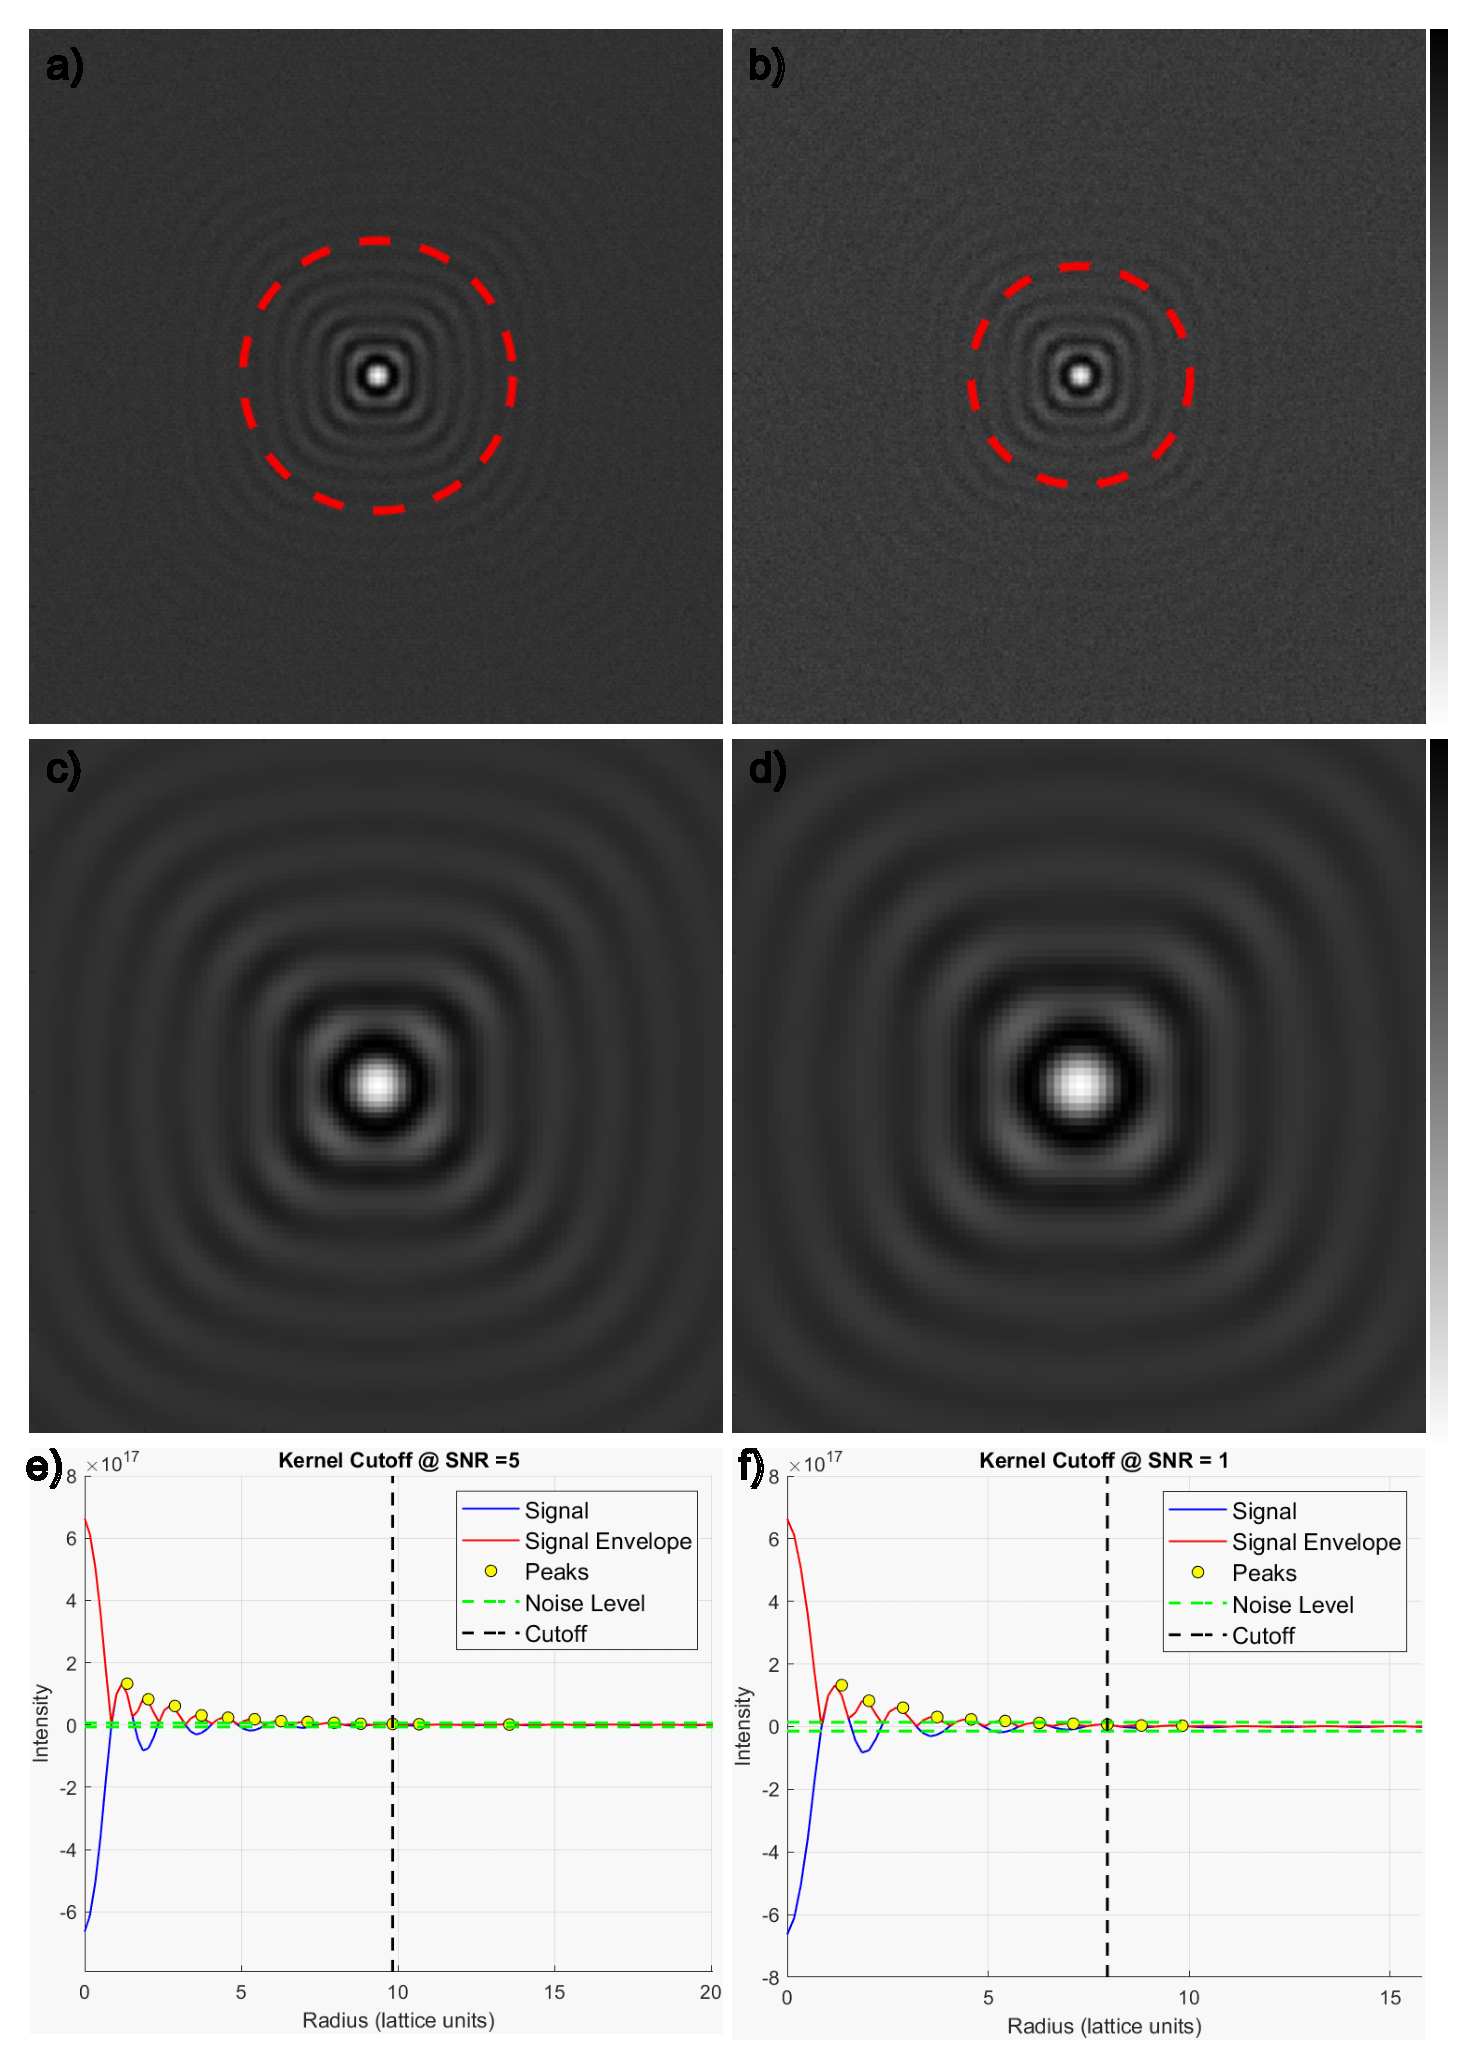
\includegraphics[width= \textwidth]{kernel_size.pdf} 
	\centering
	\caption{}
	\label{fig:ch7_kernel_size}
\end{figure}

\subsection{Tune-able parameter space}

\section{Benchmark tests on the parameter space}
\subsection{sparsity}
\subsection{Number of defect types}
\subsection{spatial resolution and noise level}

\section{MC-SBD-STM on real data}
\subsection{real data complexity}
\subsection{preprocessing pipelines}
\subsection{Ag}
\subsection{ZrSiTe}
\subsection{PtSn4}
\subsection{Potential use in other materials}
